\documentclass{article}\usepackage{multirow}\usepackage{cancel}\usepackage{changepage}\usepackage{graphicx}\title{RaTeX Physics Lab}\author{Tristan Simpson}\begin{document}\maketitle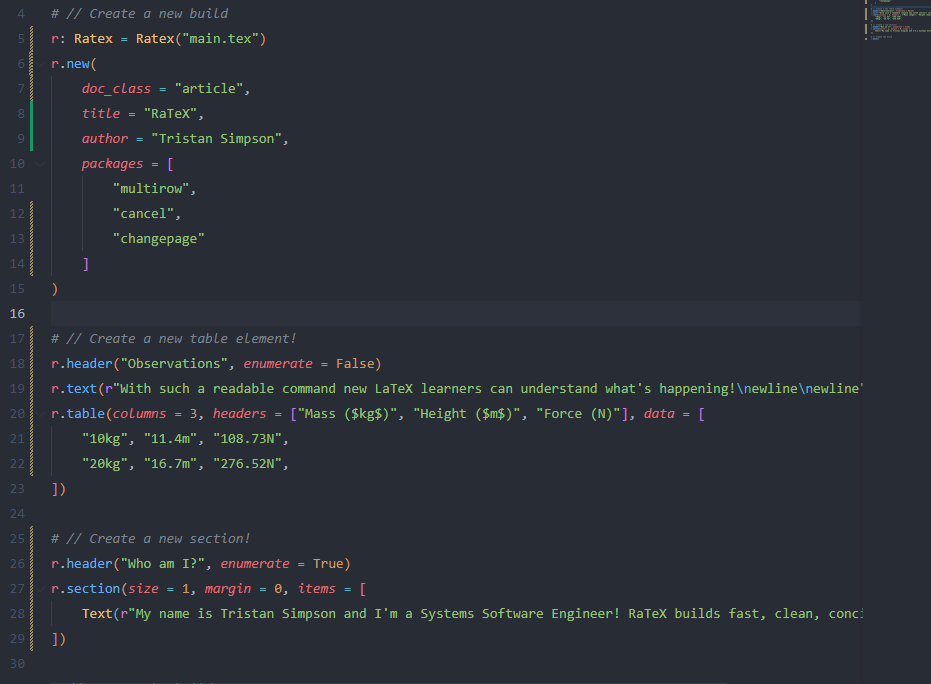
\includegraphics[scale=1]{/Users/tristan/Desktop/ratex/images/ratex1.png}\begin{itemize}\item {this}\item {is }\item {a}\item {test}\end{itemize}\leavevmode\section*{Observations}{Using the two provided object we could calculate net force of the bounceback from a mass and a string. By 30kg the string broke after the mass was dropped. The table below describes our group observations.\newline\newline}\begin{tabular}{|c|c|c|}\hline{Mass ($kg$)}&{Height ($m$)}&{Force (N)}\\\hline{10kg}&{11.4m}&{108.73N}\\\hline{20kg}&{16.7m}&{276.52N}\\\hline\end{tabular}\leavevmode\\\section*{Procedure}\begin{enumerate}\item {{The string was attached to the table.}}\item {{The mass was attached to the opposite end of the string.}}\item {{The mass was dropped and the bounceback height was measured.}}\item {{The net force was calculated.}}\end{enumerate}\leavevmode\end{document}